\scanpage{590}

\textcircled{4}\quad Cas des $\mathrm{Ind}(C)$ i.e. des \inserted{$\unsure{\mathcal U|U}$-}\unsure{paratopos|protopos} \inserted{($C$ stable par $\underset{\longrightarrow}{\lim}$ finies)} à \unsure{eng.|cog.|cond.} de prés. finie. On a

\[
\mathrm{Ind}(S)\boxtimes\mathrm{Ind}(T)\simeq\mathrm{Ind}(S\mathbin{\overset{1}{\boxtimes}}T)
\]

où

\[
\begin{aligned}
S\mathbin{\overset{\deleted{\unsure{1}}f}{\boxtimes}}T
&\mathrel{\overset{\mathrm{\unsure{déf|def}}}{=}}\bigl(\mathrm{Ind}(S)\boxtimes\mathrm{Ind}(T)\bigr)_{\mathrm{PF}}\\
&\simeq\bigl(\mathrm{Hom}^{!!f.}(S^{\mathrm o},T^{\mathrm o};\mathrm{Ens})\bigr)_{\mathrm{PF}}\\
&\hspace{7em}\cap\\
&\hspace{5em}(S\times T)^{\wedge}_{\mathrm{PF}}
\end{aligned}
\]

\uline{NB}\quad Les opérations $\unsure{\mathcal M|M}\mathbin{\overset{\unsure{\pi|\kappa}}{\boxtimes}}\unsure{\mathcal N|N}$ pour $\pi$ \unsure{cardin.|cardinal} \unsure{transfini|infini}, ou $\pi=f$, \unsure{finies|fini}, \deleted{\unsure{ou}} sur les catégories qui sont stables par $\underset{\longrightarrow}{\lim}$ de \unsure{cardinal} $\leq\pi$ (resp. par $\underset{\longrightarrow}{\lim}$ finies), est comm. à isom près, et associatif et unitaire à équiv. près. L'objet unité est $\mathrm{Ens}_\pi$ resp. $\mathrm{Ens}_f$.

\figure{\begin{tikzpicture}
\node[inner sep=0pt] (symbol) {$\unsure{\mathbb P|P}\mathbin{\underset H\wedge}\unsure{\mathbb Q|Q}$};
\node[inner sep=0pt,anchor=west,text width=.65\linewidth,align=left] (words) at ([xshift=1.8em]symbol.east)
 {si $P$ et $Q$ sont des $H$-gerbes (sur un topos) $H$ faisceau abélien. C'est une opération associative, comm., \unsure{unitaire} à \unsure{équivalence} près\ldots.};
\draw[line width=.4pt] ([xshift=-1em]symbol.west)
 .. controls +(-.15em,3ex) and +(-2em,-.3ex) .. ([yshift=.45ex]words.north west)
 .. controls +(2.2em,.3ex) and +(-.8em,.55ex) .. ([xshift=-.75em,yshift=.95ex]words.north east)
 .. controls +(1em,-.1ex) and +(.08em,1ex) .. ([xshift=.25em,yshift=.8ex]words.east);
\draw[line width=.4pt] ([xshift=-1em,yshift=-.2ex]symbol.west)
 .. controls +(.15em,-2.7ex) and +(-1.8em,.25ex) .. ([yshift=-.6ex]words.south west);
\draw[line width=.4pt] ([xshift=.3em,yshift=-.7ex]words.south)
 .. controls +(1.4em,.2ex) and +(-.7em,-.55ex) .. ([xshift=.15em,yshift=.15ex]words.south east);
\draw[line width=.35pt] ([xshift=-1.5em,yshift=2.1ex]words.north west) -- ([xshift=3.2em,yshift=2.6ex]words.north west);
\end{tikzpicture}}

% archive sheet number: 589
